\documentclass[a4paper,12pt,french]{article}

\usepackage[cours]{../../../Style}
%\geometry{bottom=1cm}
\usetikzlibrary{decorations.markings}
% Début du document
%%%%%%%%%%%%%%%%%%%
\begin{document}

\title{Variations de fonctions}
\maketitle

\begin{programme}
\item Croissance, décroissance, monotonie d'une fonction définie sur un intervalle. Tableau de variations
\item Maximum, minimum d'une fonction sur un intervalle
\item Capacités:
\begin{itemize}
\item Relier représentation graphique et tableau de variations
\item Déterminer graphiquement les extremums d'une fonction sur un intervalle
\item Exploiter un logiciel de géométrie dynamique ou de calcul formel, la calculatrice ou Python pour décrire les variations d'une fonction donnée par une formule
\end{itemize}
\end{programme}

\section{Etude des variations}

\begin{fait}%[defin]
On se donne dans cette partie $f$ une fonction définie sur un intervalle $I$.
\end{fait}

\begin{defins}
\compolignehaut
{
On dit que $f$ est croissante sur I si lorsque la variable augmente dans $I$, les images augmentent aussi. L'ordre est conservé:

\begin{center}
Pour $x,y \in I$, si $x \leq y$ alors $f(x) \leq f(y)$.
\end{center}

Graphiquement, la courbe de $f$ "monte": \nearrow
\begin{center}
\begin{tikzpicture}
\begin{axis}[
styleglobal,
width=0.9*\linewidth,
xmin=-0.5, xmax=2,
ymin=-0.5, ymax=2,
xtick distance=0.5,
ytick distance=0.5,
ticks=none,
declare function={f(\x)=e^(\x-1);}
]
\addplot[styleplot]{f(x)} node [pos=0.7,below right] {$\mathscr C_f$};
\node[stylepoint,fill=blue] (A) at (0.5,{f(0.5)}) {};
\node[stylepoint,fill=blue] (B) at (1.2,{f(1.2)}) {};
\draw[color=blue,dashed,very thick] (0.5, 0) -- (A) node [pos=0,below] {$x$} -- (0,{f(0.5)}) node [pos=1,left] {$f(x)$};
\draw[color=blue,dashed,very thick] (1.2, 0) -- (B) node [pos=0,below] {$y$} -- (0,{f(1.2)}) node [pos=1,left] {$f(y)$};
\end{axis}
\end{tikzpicture}
\end{center}
}
{
On dit que $f$ est décroissante sur I si lorsque la variable augmente dans $I$, les images diminuent. L'ordre n'est pas conservé:

\begin{center}
Pour $x,y \in I$, si $x \leq y$ alors $f(x) \geq f(y)$
\end{center}

Graphiquement,la courbe de $f$ "descend": \searrow
\begin{center}
\begin{tikzpicture}
\begin{axis}[
styleglobal,
width=0.9*\linewidth,
xmin=-0.5, xmax=2,
ymin=-0.5, ymax=2,
xtick distance=0.5,
ytick distance=0.5,
ticks=none,
declare function={f(\x)=e^(0.5-\x);}
]
\addplot[styleplot]{f(x)} node [pos=0.9,above right] {$\mathscr C_f$};
\node[stylepoint,fill=blue] (A) at (0.5,{f(0.5)}) {};
\node[stylepoint,fill=blue] (B) at (1.2,{f(1.2)}) {};
\draw[color=blue,dashed,very thick] (0.5, 0) -- (A) node [pos=0,below] {$x$} -- (0,{f(0.5)}) node [pos=1,left] {$f(x)$};
\draw[color=blue,dashed,very thick] (1.2, 0) -- (B) node [pos=0,below] {$y$} -- (0,{f(1.2)}) node [pos=1,left] {$f(y)$};
\end{axis}
\end{tikzpicture}
\end{center}
}
\end{defins}

\begin{ex}
\compo[0.67]{
On se donne la fonction $f$, définie sur $\left[1;7\right]$ et représentée ci-contre.

\begin{itemize}
\item $f$ est croissante sur $[1;4]$ puis décroissante sur $[4;7]$.
\item $f$ est croissante sur $[1;4]$ et $2 \leq 3$ donc $f(2) \leq f(3)$.
\item $f$ est décroissante sur $[4;7]$ et $5 \leq 6$ donc $f(5) \geq f(6)$.
\end{itemize}
}
{
%\vspace{-0.5em}
\begin{center}
\begin{tikzpicture}
\begin{axis}[
styleglobal,
width=1*\linewidth,
xmin=-0.5, xmax=7.5,
ymin=-0.5, ymax=3.5,
ytick distance=1,
xtick distance=1
%scale=0.7
]
\addplot[styleplot,tension=0.7] plot coordinates {(1,1) (4,3) (7,0.5)} node [pos=0.9,above right] {$\mathscr C_f$} \pointsextremites;
\end{axis}
\end{tikzpicture}
\end{center}
}
\end{ex}

\begin{defins}

\begin{itemize}
\item On dit que $f$ est constante sur $I$ si elle prend toujours la même valeur:
\begin{center}
Pour $x,y \in I$, on a $f(x)=f(y)$.
\end{center}
\item On dit que $f$ est monotone sur $I$ si elle est soit croissante, soit décroissante sur I (son sens de variation ne change pas).
\end{itemize}
\end{defins}

\rem{Exos 1,2}

\section{Tableaux de variations}

\begin{methode}
Dresser le tableau de variations de $f$, c'est indiquer sur quels intervalles la fonction $f$ est croissante, décroissante ou constante.
\end{methode}

\begin{ex}
\compo[0.4]{
%\vspace{-0.5em}
\begin{center}
\begin{tikzpicture}
\begin{axis}[
styleglobal,
width=1*\linewidth,
xmin=-3, xmax=6,
ymin=-1.5, ymax=4.5,
ytick distance=1,
xtick distance=1
%scale=0.7
]
\addplot[styleplot,tension=0.45] plot coordinates {(-2,1.5) (-1,4) (1,0) (2,-1) (4,0) (5,2)} node [pos=0.9,above left] {$\mathscr C_g$} \pointsextremites;
\end{axis}
\end{tikzpicture}
\end{center}
}
{
%\vspace{-1.5em}
On se donne la fonction $g$, définie sur $\left[-2;5\right]$ et représentée ci-contre.
On "résume" la courbe représentative de $g$ sous forme du tableau de variations suivant:
\begin{center}
\begin{tikzpicture}
\tkzTabInit[lgt=1.4,espcl=1.7]{$x$/1, $g(x)$/2}{$-2$,$-1$,2,5}

\tkzTabVar{-/1.5, +/ 4, -/$-1$, +/2 }
\end{tikzpicture}
\end{center}
}
\end{ex}

\rem{Exos 4,6,3,5,(9)}

\section{Extrémas d'une fonction sur un intervalle}

\begin{defins}
Soit $f$ une fonction définie sur un intervalle $I$.
\begin{itemize}
\item On dit que $f$ admet un maximum $M$ en $a$ sur $I$ si pour tout $x \in I, f(x) \leq M = f(a)$.
\item On dit que $f$ admet un minimum $m$ en $b$ sur $I$ si pour tout $x \in I, f(x) \geq m = f(b)$.
\end{itemize}
\end{defins}

\begin{rmq}
Le maximum d'une fonction correspond au point le plus "haut" de sa courbe représentative, et le minimum au point le plus "bas".
\end{rmq}

\begin{ex}
\compo[0.55]
{
On reprend la fonction $g$ de l'exemple précédent.

\

Son maximum sur $I$ est $4$, atteint en $-1$.

Son minimum sur $I$ est $-1$, atteint en $2$.

Son minimum sur $[-2;0]$ est $1,5$, atteint en $-2$.
}
{
\begin{center}
\vspace{-2em}
\begin{tikzpicture}
\begin{axis}[
styleglobal,
width=0.9*\linewidth,
xmin=-3, xmax=6,
ymin=-1.5, ymax=4.5,
ytick distance=1,
xtick distance=1
%scale=0.7
]
\addplot[styleplot,tension=0.45] plot coordinates {(-2,1.5) (-1,4) (1,0) (2,-1) (4,0) (5,2)} node [pos=0.9,above left] {$\mathscr C_g$} \pointsextremites;
\node[stylepoint,fill=DarkGreen] at (-1,4) {};
\node[stylepoint,fill=DarkGreen] at (2,-1) {};
\addplot[styleplot,dashed,color=DarkGreen] plot {4} node[pos=0.8,above=-2pt,color=DarkGreen!50!black] {\textbf{maximum}};
\addplot[styleplot,dashed,color=DarkGreen] plot {-1} node[pos=0.8,below=-2pt,color=DarkGreen!50!black] {\textbf{minimum}};
\end{axis}
\end{tikzpicture}
\end{center}
}
\end{ex}

\rem{Exos 7,8}

\end{document}
